\section{Обзор литературы}

Задача поиска путей с контекстно-свободными ограничениями (она же CFPQ) была сформулирована Михалисом Яннакакисом ещё в 1990 году~\cite{Yannakakis1990} в применении к запросам к декларативному языку Datalog~\cite{DatalogWiki, Ceri1989}, textit{но эта идея не была особо развита}.

В последнее десятилетие интерес к задаче \textit{вспыхнул с новой силой} в контексте запросов к RDF (Resource Description Framework)~\cite{RDF}\footnote{Среда описания ресурса}~--- графовой модели представления данных в сети, разработанной W3C (World Wide Web Consortium)\footnote{Консорциум Всемирной паутины}. RDF хранит объекты (ресурсы) и утверждения об их связях (тройки <<субъект~--- предикат~--- объект>>). Чаще всего для работы с данными, представленными в RDF, используют язык запросов SPARQL~\cite{SPARQL}. Однако SPARQL позволяет осуществлять только запросы, представленные в виде регулярных выражений, тогда как некоторые интересные запросы (такие как \textit{same-generation queries}\footnote{Запросы поиска объектов, находящихся на одном уровне иерархии}~\cite{Abiteboul1995}) могут быть выражены только в терминах контекстно-свободных языков.

Задача также нашла широкое применение в разных видах статического анализа~\cite{Reps1998} (в это области она более известная под именем задачи контекстно-свободной достижимости или CFL-Reachability), таких как 

\TODO: написать про виды стат анализа..

% In practice, widely-used large-scale analysis tools, such as Wala [Wal 2003]
% and Soot [Bodden 2012; Vallée-Rai et al. 1999], equip CFL reachability techniques to perform
% such analyses


% Тем более, некоторые из них встречаются на практике чаще остальных~\cite{Kodumal04}. 

 % К сожалению, недавно Кёйперс и др. экспериментально показали~\cite{Kuijpers19}, что текущие методы не достаточно эффективны для использования на практике. Что не удивительно, так как все они имеют асимптотику $\O(n^3)$ (где $n$~--- размер входного графа, а размер грамматики~--- константа), и лучшее ускорение, которого можно добиться, уменьшает время работы лишь в $\O(\log n)$ раз~\cite{Chaudhuri06} (используя метод четырёх русских~\cite{Arlazarov70}). Более того, существует условная нижняя оценка~\cite{Heintze1997,Chatterjee17}, согласно которой не существует комбинаторного\footnote{Этот термин не вполне определен, но можно понимать его как ``не алгебраический''. В частности, комбинаторные алгоритмы не должны использовать деление и вычитание, так те пользуются особенностями алгебраических структур (а именно, существованием обратного)} субкубического\footnote{С временем работы $\O(n^{3 - \eps})$} алгоритма для задачи CFPQ.

\subsection{Решения задачи в общем случае}

За более чем 30 лет было предложено множество алгоритмов для решения задачи CFPQ. 

Большая часть решений реализует идеи различных алгоритмов разбора выражений (парсинга). Так, алгоритм Мельски и Репса~\cite{Reps97} использует тот же подход, что и алгоритм Кока-Янгера-Касами~\cite{Younger1967} парсинга КС-языков: приведение грамматики к нормальной форме Хомского~\cite{Chomsky1957} и подсчёт динамического программирования~--- и имеет ту же асимптотику $\O(|V|^3 |N|^3)$, где $|V|$~--- число вершин в графе, $|N|$~--- число нетерминалов входной грамматики. Позднее Чаудхури~\cite{Chaudhuri06} улучшил этот алгоритм, уменьшив асимптотику в $\log |V|$ раз, используя метод четырёх русских~\cite{Arlazarov70}.

Алгоритм Григорьева и Рогозиной, основан на обобщённом нисходящем синтаксическом анализе\footnote{Top-down parsing}~--- GLL~\cite{Scott10} парсинге, и работает за $\O(|V|^3 \max\limits{v \in V} (deg^{+}(v)))$. Алгоритм Медейроса и др.~\cite{Medeiros18} также основан на нисходящем синтаксическом анализе~--- LL парсинге, но имеет время работы $\O(|V|^3 |P|)$, где $|P|$~--- число продукций входной грамматики.

Алгоритм Сантоса и др.~\cite{Santos18} основан на восходящем синтаксическом анализе\footnote{Bottom-up parsing}~--- Tomita-Style Generalized LR парсинге~\cite{Scott00}, однако его время работы не оценено (\TODO: точно?), а на некоторых входах он вообще не завершается (однако на практике показывает хорошую производительность). 

Но есть и подходы, не основанные на алгоритмах парсинга. 
Например, в своей работе Азимов и Григорьев~\cite{Santos18} сводят задачу CFPQ к транзитивному замыканию матриц (по аналогии с решением Валианта~\cite{Valiant1975} задачи распознавания КС-языков). Преимущество этого алгоритма в том, что он использует операции над матрицами, которые могут быть соптимизированы с использованием GPGPU\footnote{General-purpose computing on graphics processing units~--- техника использования графического процессора для неграфических целей (математических вычислений)}.

Хеллингс в своей работе~\cite{Hellings15} рассматривает задачу в основанной на путях (path-based) семантике запроса и разрешает её, используя аннотированные грамматики.

Чаудхури~\cite{Chaudhuri08}, а также Орачев и др.~\cite{Orachev20} сводят задачу CFPQ к задаче достижимости в рекурсивном конечном автомате, которую решают, используя инкрементальное транзитивное замыкание. Наивная реализация работает за $\O(|V|^3 |N|^3)$, но так же (как и алгоритм Репса~\cite{Reps97,Chaudhuri06}) может быть соптимизирован~\cite{Shemetova21} в $\log |NV|$ раз методом четырёх русских.

\subsection{Нижние оценки}

Как можно заметить, все существующие алгоритмы (для решения CFPQ в общем случае) имеют кубическое (или большее) время работы. Что не достаточно эффективно для работы с реальными данными, как экспериментально показали Кёйперс и др.~\cite{Kuijpers19}, реализовав и замерив производительность трёх алгоритмов: Хеллингса~\cite{Hellings15}, Сантоса и др.~\cite{Santos18} и Азимова и др.~\cite{Santos18}.

Более того, скорее всего, решения с более быстрой ($\O(n^{3 - \eps})$) асимптотикой не существует. Это так называемый ``cubic bottleneck''~\cite{Heintze1997} (узкое место) данной задачи. Было доказано, что она является 2NPDA\footnote{Языки, распознаваемые 2-сторонними автоматами с магазинной памятью (2-way nondeterministic pushdown automata~\cite{Aho1968})}-полной, и субкубическое решение для неё повлечёт наличие субкубических алгоритмов для всех задач класса. Учитывая, что такие решения не были найдены за более чем 50 лет, маловероятно, что данная задача решается быстрее куба. 

Существуют и другие условные нижние оценки. 

Так, Чаттерджи и др. в своей работе~\cite{Chatterjee17} построили условную нижнюю оценку, сведя в к задаче CFPQ (а именно, к $\cool{D}_k$-достижимости (опр.~\ref{def:dyck_reachs})) задачу BMM\footnote{Boolean Matrix Multiplication~--- перемножение двух булевых матриц}, на которую есть условная нижняя оценка. А именно, согласно BMM-гипотезе~\cite{Williams18}, не существует субкубического \textit{комбинаторного}\footnote{Этот термин не вполне определен, но можно понимать его как ``не алгебраический''. В частности, комбинаторные алгоритмы не должны использовать деление и вычитание, так те пользуются особенностями алгебраических структур (а именно, существованием обратного)} алгоритма для перемножения двух булевых матриц. Замечание про комбинаторность алгоритма важно, так как алгебраическое субкубическое решения для BMM существует, а именно, она сводится к обычному перемножению матриц, которое может быть совершено за $\O(n^{\omega})$\footnote{$\omega < 2.373$~\cite{Alman20}}.

Позднее Чжан~\cite{Zhang20} улучшил эту оценку, построив сведение BMM к $\cool{D}_1$-достижимости, тем показав, что, скорее всего, не существует субкубического комбинаторного решения уже для неё. 

И если с комбинаторными алгоритмами всё более менее понятно и оценки (нижняя и верхняя) сходятся, то с некомбинаторными всё не так радужно. Нижняя оценка в $\O(n^{\omega})$ вытекает из сведения от BMM, но обратного сведения не построено и непонятно, может ли эта оценка быть достигнута. Более того, существует условная нижняя оценка на нижнюю оценку: Чистиков и др.~\cite{Chistikov21} показали, что при условии NSETH~\cite{Carmosino16} не существует нижней оценки, основанной на SETH~\cite{Impagliazzo01} для $\cool{D}_2$-достижимости, лучшей, чем $\O(n^{\omega})$.

\subsection{Решения задачи в частных случаях}

Понятно, что для решения практических задач далеко не всегда нужна CFPQ в общем случае. Чаще всего для каждой конкретной задачи нужна конкретная КС грамматика, а иногда ещё и понятны ограничения на тип графа.

Пользуясь этой информацией (ограничениями на тип грамматики и графа) можно конструировать частные, более быстрые решения, или давать более точные оценки на время работы существующих. 

Одним из языков, для которых строятся частичные решения, является язык Дика.

% Язык Дика
\begin{definition}\label{def:dyck}
  \textit{Языком Дика} на $k$ типах скобок $\cool{D}_k$ называют язык, заданный над алфавитом $\Sigma_k = \{ (_1, )_1, (_2, )_2 \dots (_k, )_k \}$ и состоящий из правильных скобочных последовательностей на $k$ типах скобок.

  Язык Дика~--- контекстно-свободный и задаётся следующей грамматикой:\\ $D_k : S ::= S S~|~(_1 S )_1 ~|~ (_2 S )_2~|~ \dots (_k S )_k ~|~ \eps$

\end{definition}

\begin{definition}\label{def:dyck_reach}
  Задачу CFPQ для языка Дика называют также задачей Диковой достижимости (Dyck-reachability~\cite{Kodumal04}) или $\cool{D}_k$-достижимости.
\end{definition}

Задача Диковой достижимости широко применяется в статическом анализе~\cite{}, так как во многих видах анализа возникают парные объекты: вызовы и возвраты из функций (\TODO), обращение по указателю и их разыменование (\TODO), запись/чтение из поля (\TODO), взятие и возврат блокировки (\TODO).

% A Dyck language essentially
% generates well-balanced parentheses, which can be used to
% capture well-paired program properties, such as function calls/returns [15, 16, 22], pointer references/dereferences [27,
% 28], locks/unlocks [10, 13], and field reads/writes [9, 24, 25].

% https://helloqirun.github.io/papers/pldi20_yuanbo2.pdf

\TODO: Всё тут переписать

\begin{note}
  Строки, принадлежащие языку Дика $\cool{D}_1$ часто изображают в виде так называемых \textit{путей Дика}~--- путей из точки $(0, 0)$ в точку $(0, 2n)$, не опускающихся ниже оси абсцисс. Открывающей скобке соответствует вектор $(1, 1)$, закрывающей~--- $(1, -1)$.

  \TODO: Картинка 
\end{note}

% Оператор смешивания
\begin{definition}
  Для двух языков $L_1$ и $L_2$, заданных над алфавитами $\Sigma_1$ и $\Sigma_2$ соответственно, определим \textit{оператор смешивания} (interleaving operator~\cite{Li21})\\ $\odot: L_1 \times L_2 \to (\Sigma_1 \cup \Sigma_2)^{*}$ следующим образом:
  \vspace{-\topsep}
  \begin{itemize}
    \setlength\itemsep{-0.1em}
    \item $a \odot \eps = \{ a \}$, где $a \in L_1$
    \item $\eps \odot b = \{ b \}$, где $b \in L_2$
    \item $c_1 a \odot c_2 b = \{ c_1 w~|~w \in (a \odot c_2 b) \} \cup \{ c_2 w~|~w \in (c_1 a \odot b) \}$,\\ где $a \in L_1, b \in L_2, c_1 \in \Sigma_1, c_2 \in \Sigma_2$
  \end{itemize}

  Можно также переопределить оператор смешивания для двух языков:\\ $L_1 \odot L_2 = \bigcup\limits_{a \in L_1, b \in L_2} a \odot b$.
\end{definition}

%Смешанный язык Дика
\begin{definition}
  Пусть есть два языка Дика $\cool{D}_i$ и $\cool{D}_j$, заданные над разными алфавитами. Тогда назовём язык $D_i \odot D_j$ \textit{смешанным языком Дика}.

  Неформально, это множество таких скобочных последовательностей, что их проекции на алфавиты $\Sigma_i$ и $\Sigma_j$ принадлежат $\cool{D}_i$ и $\cool{D}_j$ соответственно.

  Например, для $\cool{D}_b$~--- языка квадратных ПСП и $\cool{D}_p$~--- языка круглых ПСП, $\cool{D}_b \odot \cool{D}_p$ содержит такие слова как ``\texttt{([)]}'' и ``\texttt{([()(])[])}''.
\end{definition}


\begin{definition}
  Помеченный граф $G = \q{V, E, \Sigma_k}$ называют \textit{двунаправленным} (bidirected), если в нём для каждого ребра $\q{u, v, (_i}$ найдётся противоположное ребро $\q{v, u, )_i}$ и наоборот.

  Неформально, матрица смежности такого графа симметрична, и метки на симметричных рёбрах~--- это парные открывающая/закрывающая скобки.
\end{definition}

\begin{enumerate}
    \item Язык Дика $\O(n^3 k)$ \cite{Kodumal04}

    Просто применить алгоритм Репса \cite{Reps97} и нормально оценить время работы.

    \item Язык Дика (почти) $\O(n^3)$ \cite{Rehof01}

    Ещё более точный анализ алгоритм Репса \cite{Reps97}, учитывающий, что построенный (для конкретного анализа) граф содержит константное число скобок

    \item Язык Дика на одном типе скобок $D_1$ $\O(n^{\omega} \log^2 n)$ \cite{Mathiasen21}

    Ищем bell-shaped пути: удваиваем рёбра, ищем пути с серединкой из bell-shaped пути поменьше (так $\log n^2$ раз).

    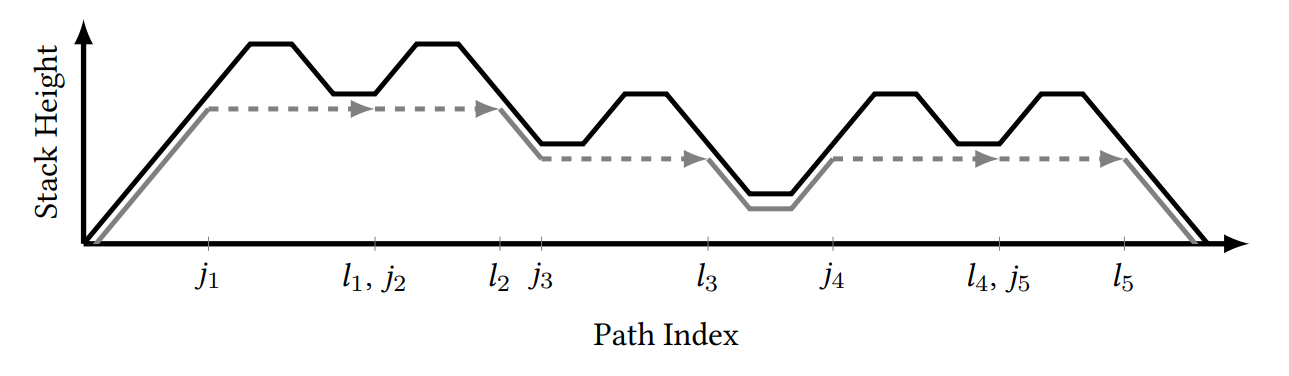
\includegraphics[width=0.75\linewidth]{img/dyck1_path.png}

    Сжимаем bell-shaped пути в $\eps$-рёбра. Снова ищем и снова сжимаем. После каждого сжимания мы убираем все локальные максимумы. Чем больше был максимум, тем длиннее $\eps$-ребро. Хуже всего, когда все новые рёбра длины 2. В любом случае путь становится короче хотя бы в 2 раза, так что таких итераций потребуется не более $\log n^2$ (есть лемма, что найдётся путь длины не более $\O(n^2)$). 

    \item Двунаправленные графы и язык Дика

    Существует несколько частных решений для задачи Диковой достижимости на двунаправленных графах:

    \begin{itemize}
        \item Деревья \cite{Yuan09}

        $\O(n \log n \log k)$~--- центроиды + внутри что-то идейное

        \item Общий случай \cite{Chatterjee17}

        Решение основано на двух фактах. Первый: в двунаправленном графе формируются компоненты Диковой достижимости. Второй: если есть две вершины $u, v$ и компонента Диковой достижимости $C$, такие что $u \xrightarrow{\alpha_i} C$ и $v \xrightarrow{\alpha_i} C$, то $u$ и $v$ тоже лежат в одной компоненте Диковой достижимости. 

        Пользуясь этими фактами, алгоритм с помощью СНМ'а поддерживает компоненты Диковой достижимости и исходящие из них рёбра, чтобы быстро искать новые пары вершин, принадлежащих одной компоненте.

        Итоговая асимптотика алгоритма $\O(m + n \alpha(n))$.
    \end{itemize}

    \item Interleaved Dyck-reachability

        Алгоритм за $\O(n^7)$ для $D_1 \bigodot D_1$ достижимости на bidirected графах~\cite{Li21}

        \textit{Там $\O(n^7)$, потому что авторы~--- дурачки, не умеют рёбра в графе посчитать}

        \textit{Ну или я дурачок, там одно из двух}

        \textit{Было ещё про это (там, вроде, про один из языков сказали, что он bounded, поэтому можно пересекать с регулярным): 
        \url{https://dl.acm.org/doi/pdf/10.1145/3296979.3192378}}
        \TODO: \textit{надо прочитать, что там пишут...}

    \item Граф-цепочка $\O(n^{\omega})$ \cite{Valiant1975}

        CFPQ на графе-цепочке~--- просто задача КС-распознавания (CF-recognition). А она решается за перемножение булевых матриц \cite{Valiant1975}

    \item Ацикличный граф $\O(n^{\omega})$ \cite{Yannakakis1990}

        Ацикличный граф~--- это почти бамбук (= цепочка), нужно только его потопсорить (и где-то ещё быть аккуратным, я не совсем помню сведение)

    \item Bounded-stack RSM $\O(n^3 k^3 / \log^2)$ \cite{Chaudhuri08}

        RSM, который не уходит в рекурсию (т.е. есть из конца ребра $\xrightarrow{S}$ не достижимо никакое ребро $\xrightarrow{S}$)

        Тут применяется какое-то более хитрое (я ещё не разбиралась) итеративное транзитивное замыкание (что-то с dfs'ом, а потом ещё 4 русских сверху, кажется)

    \item Hierarchical FSM $\O(n^{\omega} k^{\omega})$ \cite{Chaudhuri08}

        RSM, в котором боксы упорядочены (топсорт) и бокс с меньшим номером содержит рёбра только с вызовами боксов с большим номером. Задают регулярный язык, но размер FSM может быть экспоненциальным относительно размера RSM.

        Алгоритм идёт в порядке, обратном топсорту, и считает транзитивное замыкание внутри бокса, чтобы провести все рёбра, которые ему соответствуют.

\end{enumerate}

% \subsection{Вычислительная сложность}

% \TODO

% https://arxiv.org/pdf/2007.05569.pdf


\subsection{Выводы и результаты по главе}

\TODO